\documentclass[times, utf8, zavrsni]{fer}
\usepackage{booktabs}
\usepackage{float}

\begin{document}

% TODO: Navedite broj rada.
\thesisnumber{000}

% TODO: Navedite naslov rada.
\title{Web-aplikacija za rješavanje programskih zadataka s elementima društvene mreže}

% TODO: Navedite vaše ime i prezime.
\author{Nikola Kešćec}

\maketitle

% Ispis stranice s napomenom o umetanju izvornika rada. Uklonite naredbu \izvornik ako želite izbaciti tu stranicu.
\izvornik

% Dodavanje zahvale ili prazne stranice. Ako ne želite dodati zahvalu, naredbu ostavite radi prazne stranice.
\zahvala{Srdačno se zahvaljujem svojem mentoru, prof. dr. sc Igoru Mekteroviću na cijenjenoj pomoći, savjetovanju i stručnom usmjeravanju. Također se zahvaljujem i Hermanu-Zvonimiru Došiloviću na pomoći i uputama oko Judge0-a bez kojeg ovaj završni rad ne bi bio moguć.}

\tableofcontents

\chapter{Uvod}
Sveprisutnost računalnih sustava tijekom početka drugog tisućljeća uveliko je doprinijela većem porastu zanimacije populacije prema svemu što je povezano s računalima.  Naravno, to podrazumijeva i čin \textbf{programiranja}. Programiranje možemo opisati kao čin dizajniranja i razvoja izvršnog računalnog programa čija je svrha uspješno postizanje specifičnog računskog rezultata ili odrada specifičnog zadatka.\\
Iako su već početkom tisućljeća računalni sustavi bili poprilično sveprisutni, neusporedivo je koliko je njihova zastupljenost u svakodnevnom ljudskom životu porasla. Porastom njihove zastupljenosti porasla je potražnja za računalnom sklopovskom podrškom \engl{hardware}, a s njom i potreba za kvalitetnom programskom podrškom \engl{software}. Kvalitetna programska podrška rezultat je godina učenja, razmatranja i pisanja programskog koda, a kao i svaku drugu vještinu potrebno ju je održavati. Održavanje je moguće na mnogo načina, a među popularnijim načinima usavršavanja i održavanja vještosti pisanja programskog koda jest rješavanje programskih zadataka te potom rangiranje tih rješenja, a česta je i situacija da se provode i događanja gdje se sudionici natječu u kvaliteti programskih rješenja.\\
Zainteresirana neiskusna populacija teško da će svojevoljno ući na opisana događanja jer dobar je dio sudionika koji sudjeluju na takvim događanjima već vrlo vješt. Stoga je pojava internetskih stranica koje pružaju uvid u programiranje i rješavanje programskih zadataka dobrodošla novost. Ipak, često riječ iskusnog programera neiskusnom programeru može biti neprocjenjiva. Iz tog razloga zanimljiv bi bio spoj internetskih stranica koje pružaju socijalne usluge, takozvane socijalne mreže \engl{social networks} i stranica koje pružaju mogućnost rješavanja programskih zadataka. Osobi koju pisanje programskog koda interesira stranica bi pružila nekompetitivnu mogućnost rješavanja zadataka, a iskusnom programeru mogućnost da kroz rješavanje i objašnjavanje svojih rješenja produbi i utemelji svoja znanja. Upravo je takva kombinacija osnovnih elemenata stranica socijalnih mreža i stranica s tematikom programskog koda tema ovog završnog rada.

\chapter{Korisnički zahtjevi}
Internetska stranica koja kombinira elemente socijalnih mreža i elementa stranica s tematikom programskog koda treba omogućiti korisniku ispunjavanje elementarnih zahtjeva koje socijalne mreže i stranice s tematikom programiranja pružaju. Budući da skoro pa uvijek socijalne mreže traže da njihovi korisnici prvo naprave korisnički račun da bi im pristupili, na korisnika se gleda na dva načina: \textbf{neregistrirani korisnik} i \textbf{registrirani korisnik}. 
\section{Zahtjevi neregistriranog korisnika}
Neregistriran korisnik, prema uzoru na mnoge moderne socijalne mreže, ima mogućnost pristupanja samo stranici dobrodošlice te imati pravo registriranja. Grafički prikaz zahtjeva prikazan je na slici \ref{fig:zahtjevi-nereg}.

\begin{figure}[H]
	\centering
	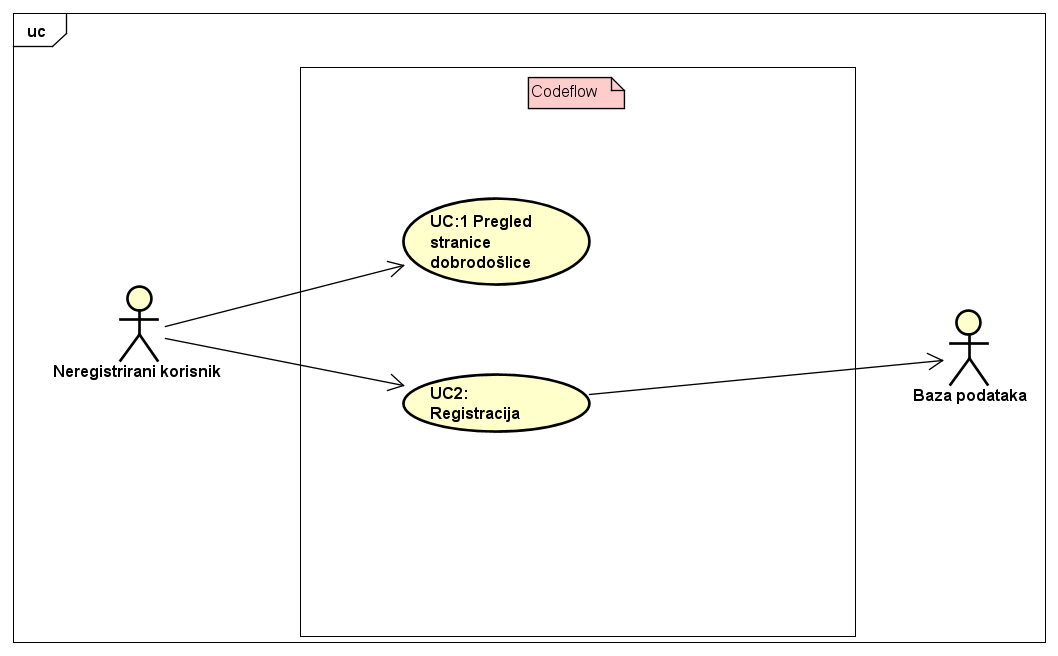
\includegraphics[width=14cm]{pictures/zahtjevi/nereg_korisnik.png}
	\caption{Zahtjevi neregistriranog korisnika}
	\label{fig:zahtjevi-nereg}
\end{figure}

\section{Zahtjevi registriranog korisnika}
Nakon što se korisnik registrira broj zahtjeva koje stranica korisniku treba ispuniti raste. Registriranom korisniku mogućnost prijave s podacima koje je koristio za registraciju mora biti omogućena te pošto se prijavi opcija pregledavanja ponuđenih zadataka i rang liste treba biti podržana. Ponuđene zadatke treba moći filtrirati na neki od ponuđenih načina i aplikacija registriranom korisniku treba nuditi mogućnost detaljnijeg pregleda pojedinog odabranog zadatka. Tijekom detaljnijeg pregleda pojedinog zadatka registriranom korisniku moraju biti ponuđene opcije ocjenjivanja i komentiranja zadatka. Uz sam detaljniji opis zadatka, korisniku treba biti omogućen odabir nekog od rješenja gledanog zadatka. Odabrano rješenje registrirani korisnik također mora moći komentirati i ocijeniti. Osim što smije pregledavati rješenja, registriranom korisniku aplikacija treba omogućiti rješavanje zadatka, tj. pisanje programskog rješenja. Njegovo rješenje aplikacija mora evaluirati pomoću vanjskog izvršitelja programskog koda te spremiti. Uz stvaranje rješenja programskih zadataka, aplikacija registriranom korisniku treba ponuditi i opciju stvaranja programskog zadatka. Registrirani korisnik mora imati mogućnost potpunog upravljanja vlastitim zadacima, rješenjima, komentarima i ocjenama. Treba mu biti omogućeno njihovo uređivanje i brisanje. Uz mogućnost upravljanja vlastitim zadacima, rješenjima, komentarima i ocjenama, registriranom korisniku mora biti omogućeno mijenjanje vlastitih podataka. Po uzoru na određene mogućnosti modernih socijalnih mreža, registriranom korisniku opcija pregleda profila drugih registriranih korisnika treba biti podržana, a potom moguće praćenje ili otpraćivanje željenih korisnika također treba biti dopušteno. Osim što podržavanje mogućnosti gledanja tuđih korisničkih stranica mora biti podržano, registrirani korisnik treba moći vidjeti svoju korisničku stranicu. Detaljniji grafički prikazi ovih korisničkih zahtjeva vidljivi su na slikama \ref{fig:zahtjevi-korisnik1} i \ref{fig:zahtjevi-korisnik2}.

\begin{figure}[htb]
	\centering
	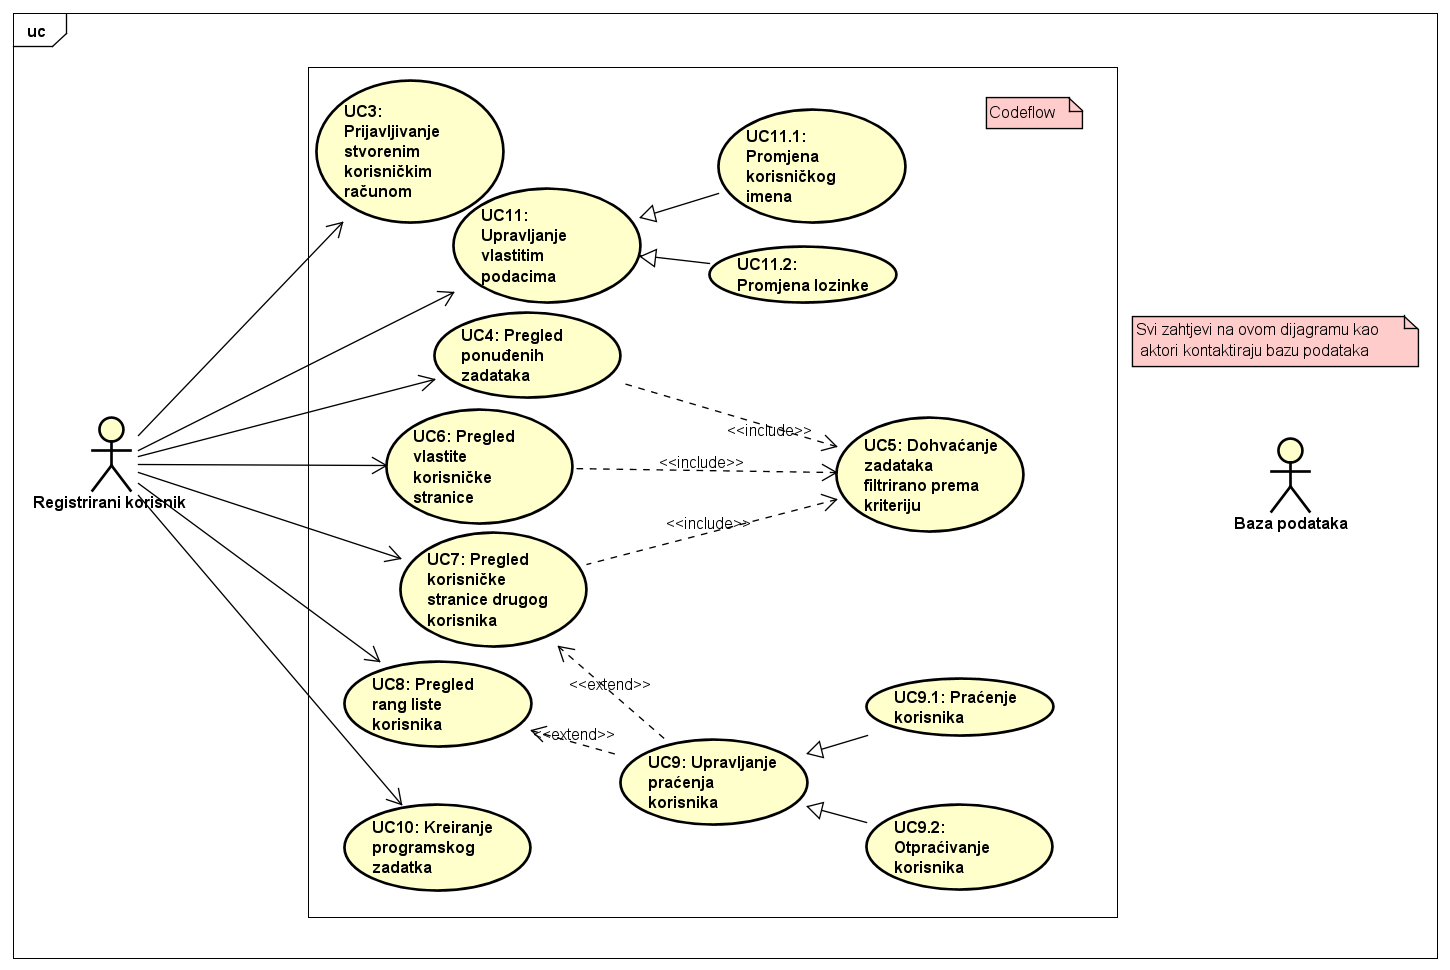
\includegraphics[width=17cm]{pictures/zahtjevi/korisnik1.png}
	\caption{Zahtjevi registriranog korisnika, prvi dio.}
	\label{fig:zahtjevi-korisnik1}
\end{figure}

\begin{figure}[htb]
	\centering
	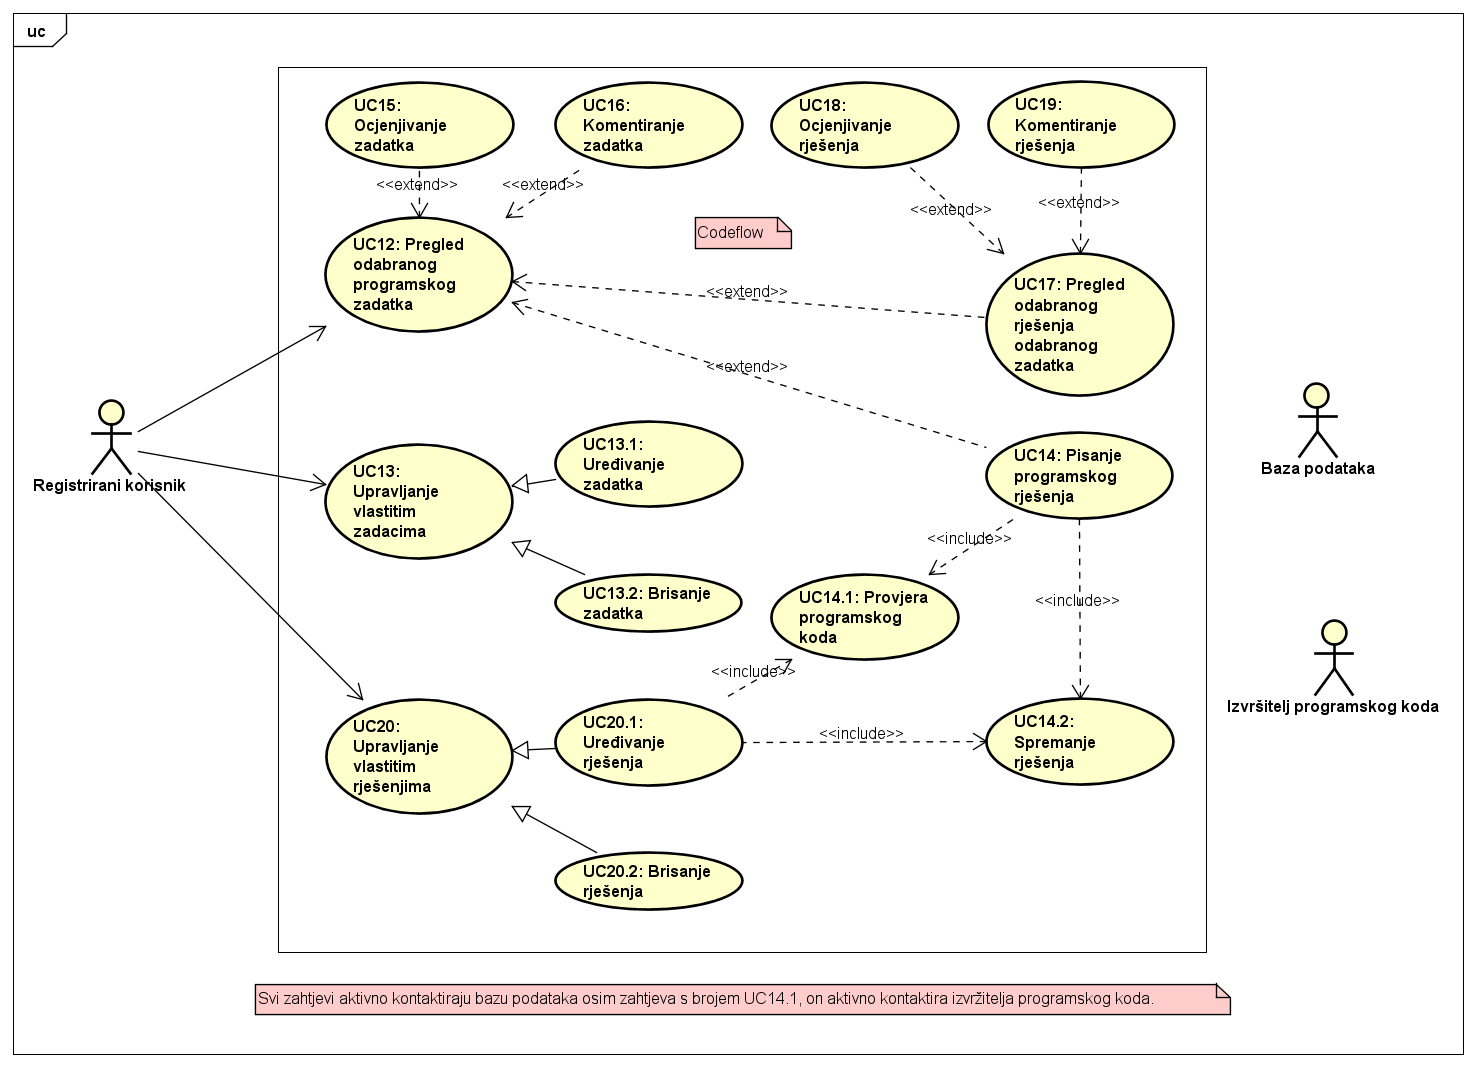
\includegraphics[width=17cm]{pictures/zahtjevi/korisnik2.png}
	\caption{Zahtjevi registriranog korisnika, drugi dio.}
	\label{fig:zahtjevi-korisnik2}
\end{figure}

\chapter{Postojeća programska rješenja te uvođenje socijalnih elemenata}
Već postojeća rješenja, njihove značajke te uvođenje socijalnih elemenata

\chapter{Korištene tehnologije}
Već postojeća rješenja, njihove značajke te uvođenje socijalnih elemenata

\chapter{Pomoćne tehnologije}
Već postojeća rješenja, njihove značajke te uvođenje socijalnih elemenata

\chapter{Arhitektura rješenja}
Već postojeća rješenja, njihove značajke te uvođenje socijalnih elemenata

\chapter{Prikaz rješenja}
Već postojeća rješenja, njihove značajke te uvođenje socijalnih elemenata

\chapter{Budući razvitak}
Već postojeća rješenja, njihove značajke te uvođenje socijalnih elemenata

\chapter{Zaključak}
Zaključak.

\bibliography{literatura}
\bibliographystyle{fer}

\begin{sazetak}
Sažetak na hrvatskom jeziku.

\kljucnerijeci{Ključne riječi, odvojene zarezima.}
\end{sazetak}

% TODO: Navedite naslov na engleskom jeziku.
\engtitle{Title}
\begin{abstract}
Abstract.

\keywords{Keywords.}
\end{abstract}

\end{document}
